% chapter 2
\chapter{Context}
In this chapter, we will discuss the related works and the relevant concepts that will help the reader understand the ideas
mentioned in this project.

\section{Related Works}
A few studies on the comparison of constraint programming solvers have been done before.
Meindl et al (2012) \cite{Meindl2012} conducted a study on the analysis of popular commercial and open source solvers and concluded
that IBM's CPLEX\footnote{See \url{http://www-01.ibm.com/software/commerce/optimization/cplex-optimizer/}} has the best performance,
followed by Gurobi\footnote{See \url{http://www.gurobi.com}}. Hakan (2012) \cite{Hakan2012} analysed the features of
LP Solvers, including or-tools\footnote{See \url{https://developers.google.com/optimization/}}.
 He stated that or-tools has a lot of advantages such as easy of modelling problems and
active user community. Gurobi Optimization also have carried out comparative study on its tools against other open
source solvers \cite{gurobi:solvers}. The study concludes that Gurobi outperforms the other solvers mentioned.

\section{Linear Programming}
Linear programming (LP) is a mathematical method to obtain the optimal solution of a function in a linear system under set of constraints
imposed on its variables. It is a method commonly used in solving combinatorial optimisation problems in applied mathematics and operations research.
A problem is considered a linear program when all of its mathematical relationship are linear \cite{APMBradley}.
The word 'programming' is not to be confused with the term used in computer science,
in which concerns with creating instructions for computers to execute. A linear
program consists of three entities \cite{LPChvatal,ILPCoursera}:
\begin{enumerate}
\item \textbf{Decision variables} - These are the entities that can be controlled by the decision maker.
\item \textbf{Objective function} - This is the function that, given the optimal input, outputs the optimal value.
In most cases, it is to find the minimum or the maximum value.
\item \textbf{Variable constraints} - These are the restrictions that are imposed on the decision variables. There are two types
of constraints: hard and soft. Hard constraints are constraints cannot be violated at all cost, whereas soft constraints may be
violated, but should be observed wherever possible.
\end{enumerate}

To fully understand LP, it is best to look at an example: Bob is competing in
an eating contest that lasts one hour where the objective is to accumulate as much points as possible by eating a combination of hotdogs and burgers.
For each burger and hotdog that Bob eats, he will get 5 and 4 points respectively. It takes him 3 minutes to finish a burger and
2 minutes to finish a hotdog. Bob can consume 25 food items before his appetite reaches its limit.

Based on the scenario above, we can model this problem in the form of a linear program by following these steps:
\begin{itemize}
\item \textbf{Step 1}: Identify the decision variables. Let \(x\) be the number of hotdogs and \(y\) be the number
of burgers eaten by Bob.
\item \textbf{Step 2}: Determine the objective function. In this scenario, we want to determine the highest possible
points that Bob can achieve in the competition. This can be represented by the equation \(z = 4x + 5y\), where
z is the value of the points accumulated in the competition and the coefficients of the variables represent the points achieved by eating respective
food items.
\item \textbf{Step 3}: Determine the constraints. There are 3 constraints in these problem. Firstly, The amount of
food eaten by bob has to be under 60 minutes. This can be represented by the equation \(2x + 3y \leq 60\). Secondly,
Bob's appetite has a limit of 25 food items, which can be modelled with the equation \(x + y \leq 25\). Lastly,
the number of respective food eaten has to be greater than or equal to 0.
\end{itemize}
Putting them together, we have the following linear program:
\[
  \begin{array}{r@{}r@{}l}
    \text{Maximise z =} \quad &{}4x + 5y \\[\jot]
    \text{Subject to}\qquad &{} 2x +   3y &{} \leq 60 \\
    \qquad &{} x +   \phantom{2}y &{} \leq 25 \\
    \qquad &{} x ,   \phantom{2}y &{} \geq 0 \\
  \end{array}
\]
There are two types of solution that can be produced. A feasible solution is a set of variables that satisfies the constraints
of a linear program. An example of a feasible solution for the above solution would be \(x = 25\) and \(y=0\), which yields 100 points.
The goal of the linear program is to achieve optimal solution of the objective function \cite{LPChvatal}. The optimal solution is the best feasible solutions.
For the problem above, the optimal solution is 110 points, which is produced when \(x = 15\) and \(y = 10\). The feasible solutions
are bound within the feasible region marked in green as shown in Figure 2.1. The red region is the infeasible region, where any point that falls within it will not satisfy the
constraints of the linear program. The dimensions of the graph is determined by the number of variables the linear program has.
So, a linear program with three variables can only be described with three dimensional graph.

There are three types of outcomes \cite{LPChvatal,ILPCoursera} in a linear program and they are determined by the
its feasible region. The three outcomes are:
\begin{itemize}
\item \textbf{Outcome 1} : The feasible region is unbounded, thus the objective function is infinity.
\item \textbf{Outcome 2} : The feasible region is empty, this is usually because the constraints on the variables contradict each other.
\item \textbf{Outcome 3} : The feasible region is bounded. In this case, an optimal solution exists.
\end{itemize}

\begin{figure}[!ht]
  \centering
    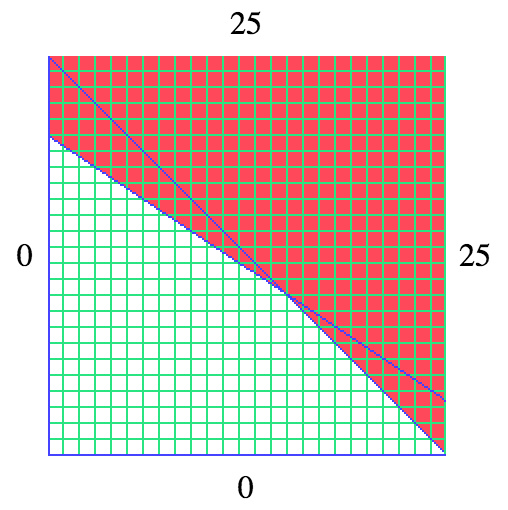
\includegraphics[width=0.5\textwidth]{example-graph.png}
    \caption{Graphical representation of the linear program example. Figure taken from \url{http://www.zweigmedia.com/}\cite{zweigmedia}}
\end{figure}

To find the optimal solution, we use the simplex method \cite{LPChvatal, LPVanderbei}.
The simplex method finds an optimal point by moving from point to point until it finds the best one.
It starts off by selecting a point in a graph.
Then it moves to a different point of the graph. On each move, it will make sure that the point yield higher
objective value. The algorithm stops when it is unable to find a point with higher objective value.
Simplex only works when the linear program has a bounded feasible region. The illustration of this algorithm is shown in figure 2.2.
For the complete explanation on the simplex method, refer to these books \cite{LPChvatal, LPVanderbei}.
\begin{figure}[!ht]
  \centering
    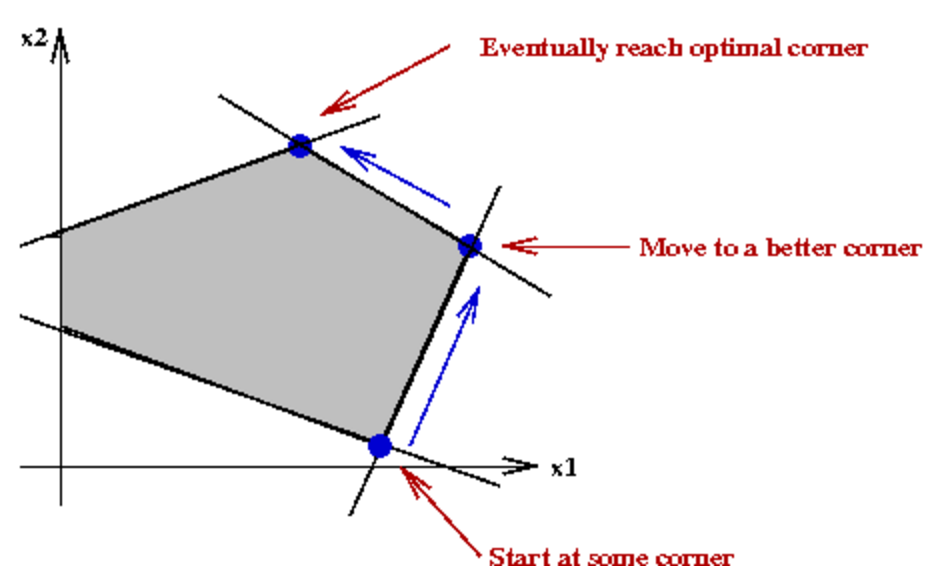
\includegraphics[width=0.8\textwidth]{simplex2.png}
    \caption{Simplex method on a linear program, taken from George Washington University \cite{seas:SM}}
    \vspace{1cm}
    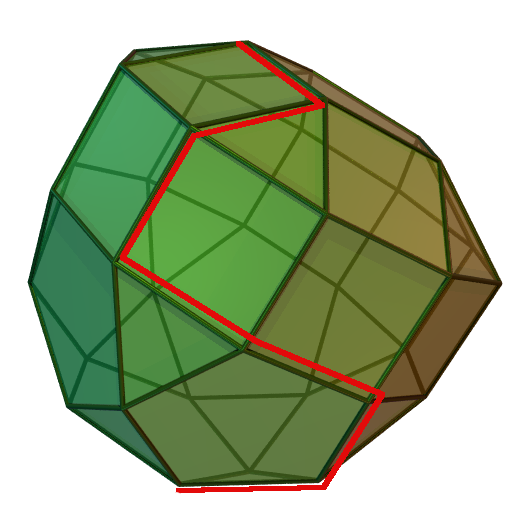
\includegraphics[width=0.5\textwidth]{simplex3d.png}
    \caption{Simplex algorithm on a 3D space, taken from Wikipedia \cite{Wiki:SPM}}
    \vspace{1cm}
\end{figure}

\section{Integer Programming}
Integer programming (IP) \cite{LPVanderbei} is LP that has an additional
integrality constraint of imposed on to its decision variables. This is useful in situations where the variables need to be
discrete, such as variables representing the number of people or boolean values.
When this constraint is added, finding an optimal solution becomes harder, as denoted by its complexity.
IP problems are in the NP Class \cite{Papadimitriou1981}, whereas LP problems are in the P class \cite{Megiddo1987}.
 IP is harder because the solution space is reduced to
the lattice points of feasible region, thereby adding more complexity in identifying the feasible solutions.
Linear programming that has both real valued and integer valued constraints on its
 decision variables is called Mixed Integer Programming (MIP) \cite{LPVanderbei}.
\begin{figure}[!ht]
  \centering
    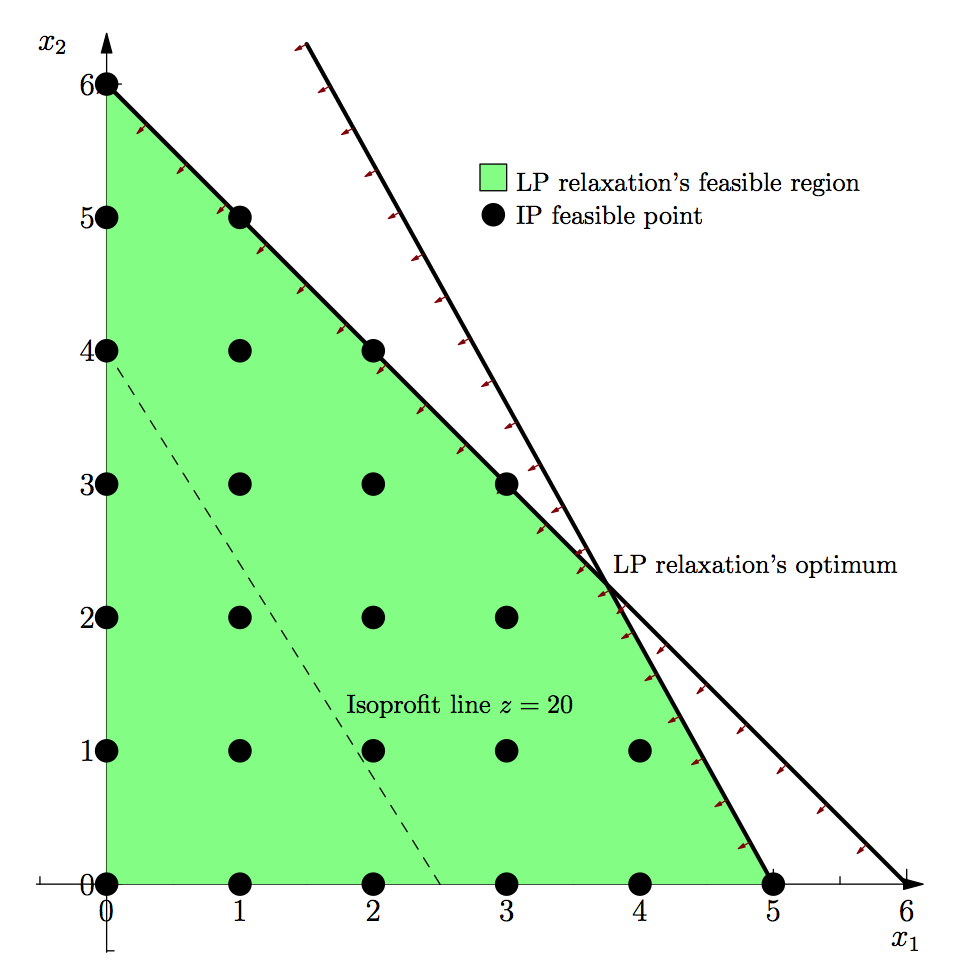
\includegraphics[width=0.7\textwidth]{ipfeasible.png}
    \caption{Feasible solutions of an integer program marked by the black dots (lattice points) bounded by the feasible region (green region), taken from
     Linear Programming: Foundations and Extensions by Robert Vanderlei \cite{Sottinen2009}}
\end{figure}

More sophisticated algorithms have been invented in order to accomodate the added complexity of IP. One of the most commonly
used algorithm that uses exact approach to finding a solution is the branch-and-bound algorithm  \cite{LPVanderbei, LPChvatal, Dastghaibifard2008}. It uses divide and
conquer approach to partition the problem into sub-problems
and then solves them recursively. LP methods such as the simplex can be used to solve the sub-problems \cite{Dastghaibifard2008}.
The 'branching' part generates a tree
that continues to expand until all valid solutions are found. The bound part compares all solutions and keeps the
most optimal one.

\section{Constraints Programming}
Unlike the programming that we have observed so far, constraints programming (CP) is a programming paradigm that is implemented
in LP solvers \cite{wiki:cp}. It is a programming paradigm that combines declarative and procedural paradigm \cite{wiki:cp, Bockmayr2003}.
The goal of CP is to find feasible solutions out of large solutions space, making it
more suitable to accomodate LP. CP focuses on the constraints and variables rather than the objective function.
In this paradigm, a constraint program may be written declaratively but should be viewed as a procedure that operates on a
solution space. Each constraints will be added to a constraint store, which limits the space that must be searched.
Constraint store uses a filtering algorithm that serves as a litmus test to determine the feasibility of a solution \cite{Bockmayr2003}.
At the end of the filtering procedure, we obtain a feasible solution.

\section{Tools}
In this project, we will be using three LP tools: Gurobi\footnote{See \url{http://gurobi.com}},
or-tools\footnote{See \url{https://developers.google.com/optimization/}} and Optaplanner\footnote{See \url{http://www.optaplanner.org}}.
We have chosen Gurobi mainly due to its performance and popularity. Or-tools and Optaplanner were chosen because
their performance have not been widely documented and they show and they show a lot of promise given their active user community
and high development activity.

Gurobi is a optimisation tool built for solving LP based problems. Its LP solver is written in C and it comes with
application programming interfaces (API) to port many different programming languages including Java, C++, Python and a few others. Gurobi allows you
to build any models for any LP problem, giving users full control to implement any algorithms or heuristics that they
prefer. It claims to be the fastest solver amongst 3 other open source solvers \cite{gurobi:solvers}, none
of which are used in this project. Gurobi is one of the most expensive commercial LP solver in the industry
and its used by many corporations such as FedEx, Netflix and Google. Academic licenses is also available for universities
and its affiliated individuals for free.

or-tools by Google is an optimisation suite for solving various optimisation problems, including VRP. It contains a constraint programming
solver, unified interface for other solvers (e.g Gurobi, GLPK, etc), implemented mostly in C++. Like Gurobi, it also comes with APIs
to support other major programming languages, albeit in less variety. This tool allows to focus on modelling the problem at hand, without worrying
too much about the algorithms and the heuristics, as they have been implemented and packaged with the solver. It is an open souce
software that is used in internally at Google that offers various advantages such as: high quality, portability and active user community.

Optaplanner is an constraint programming engine built in Java for solving optimisation problems. Unlike the other two solvers, it does not
have API to support other languages. In addition, it takes the input in the form of XML file, which are then processed by the engine. It has
predefined XML tags used to model various problems and built-in implementation of algorithms and heuristics for solving them. What Optaplanner
lacks in portability, it makes it up in usability. The XML input format allows users to define the problem rather than implementing the procedures
to solve the problem. In addition to usability, it comes with a graphical user interface (GUI) that visualise common optimisation problems, including the VRP.

\section{Graph Theory}
In this section we discuss some relevant terminologies \cite{wilson1996} from graph theory to get a better understanding of
the ideas discussed in the vehicle routing problem:
\begin{itemize}
\item A \textbf{graph} is a collection of points connected by lines in a plane. The points and lines are
more commonly refered to as \textbf{vertices} and \textbf{edges} respectively.
\item A \textbf{directed} graph is a graph whose edges goes in one direction but not the other.
\item An \textbf{undirected} graph has edges that goes in both directions.
\item A \textbf{complete} graph where all of its vertices are connected to one another.
\item A \textbf{walk} is a sequence of vertex and edges that connects one vertex to another in a graph.
\item A \textbf{path} is a walk in which no vertex appers more than once. It is also more commonly refered to as a \textbf{hamiltonian path}.
\item A \textbf{cycle} is a walk such that the first vertex corresponds with the last.
\item A \textbf{hamiltonian cycle} is hamiltonian path that also happens to be a cycle.
\end{itemize}

\section{Solution Methods and Complexity of VRP}
Solution methods come in two categories: exact approaches and heuristics. Exact approaches attempt
to find the optimal solution and will not stop until it finds one of the best \cite{neo:exact}. Some examples
include branch-and-bound \cite{LPVanderbei} and the branch-and-cut algorithm \cite{ILPCoursera}. On the other hand, heuristics approach
 attempts to solve a problem more quickly at the expense of optimality and precision. Heuristics attempts to obtain the optimal solution by incrementally improve
 the current solution \cite{Laporte1999}. We use this technique in
solving problems that may take too long to compute the exact answer or when exact algorithms failed to find any solution \cite{neo:exact}.

Lenstra et al states that all variants of VRP are NP-Hard \cite{Lenstra1981}. The implication of this is that it may
take a really long time to compute certain instances of VRP. Thus, heuristics based approach may be preferrable as opposed to
the exact one.

\section{Review}
In this chapter, we have introduced the related works and the key concepts of this project. Linear programming is a
mathematical method concerns with finding an optimal value of a function in a linear system under a set of constraints. Integer
programming is linear programming with the additional constraint where all of its decision variables are restricted to integers.
There are several algorihtms to find the optimal value of the objective function in a linear program such as simplex and branch-and-bound
algorithm. We also explained constraints programing, a programming paradigm to solve linear programs and
some background information on LP tools used in this project. We also covered some basic
concepts in graph theory that will be mentioned quite frequently throughout the project. Lastly, we discussed the
computational complexity and how it impacts the computation of VRP.

In the next chapter, we will create LP formulations and produce the requirements and the deliverables for the company involved.